\subsection{研究目标}\label{ch2target}

由于现有针对深度学习模型的测试方法可解释性不足,测试人员无法根据测试结果对深度学
习模型进行诊断和调试,用户也很难根据测试结果对模型产生足够的信任。针对这一问题,
传统基于人工(专家)分析的方法可以对深度学习模型的测试结果进行解释,但是,基于人
工分析的测试解释方法受限于专家知识,并且会产生显著的人工费用和时间开销。面对大量
测试数据,单纯的依靠人工分析获得可解释的测试反馈,可行性有限,而现有的解释性方法
与可解释的深度学习模型测试之间还存在不小的距离。面向深度学习模型测试的可解释性不足这
一显著问题,\textbf{本项目的研究目标是:提出一种自动化的、可解释的深度学习模型测
试方法,能够在不同测试场景下建立具有语义逻辑的测试覆盖指标,辅助测试人员诊断和调
试模型,并对测试集的测试逻辑进行准确的解释和说明,从而提高深度学习模型测试的
可信度。}本项目的研究工作对于深度学习应用的开发人员、测试人员和用户来说具有重要
的应用价值,对智能软件(如自动驾驶软件)的测试研究、可信软件的研究和人工智能的可
解释性研究具有重要意义。

\subsection{研究内容}\label{ch2content}

针对深度学习模型的可解释测试方法研究,如\Cref{fig:ch2:yjnr}所示,本项目拟展开
    \textbf{可解释测试覆盖指标研究和可解释测试集生成技术研究}两方面主要研究内容,
    每个研究内容又包含了多个关键技术点的研究。通过这两个核心方面的技术研究,完
    成自动化的、可解释的深度学习模型测试方法的设计与实现。以下针对这两个方面的研
    究内容进行相应的描述和解释。

\begin{figure}[htp]
    \begin{small}
        \begin{center}
            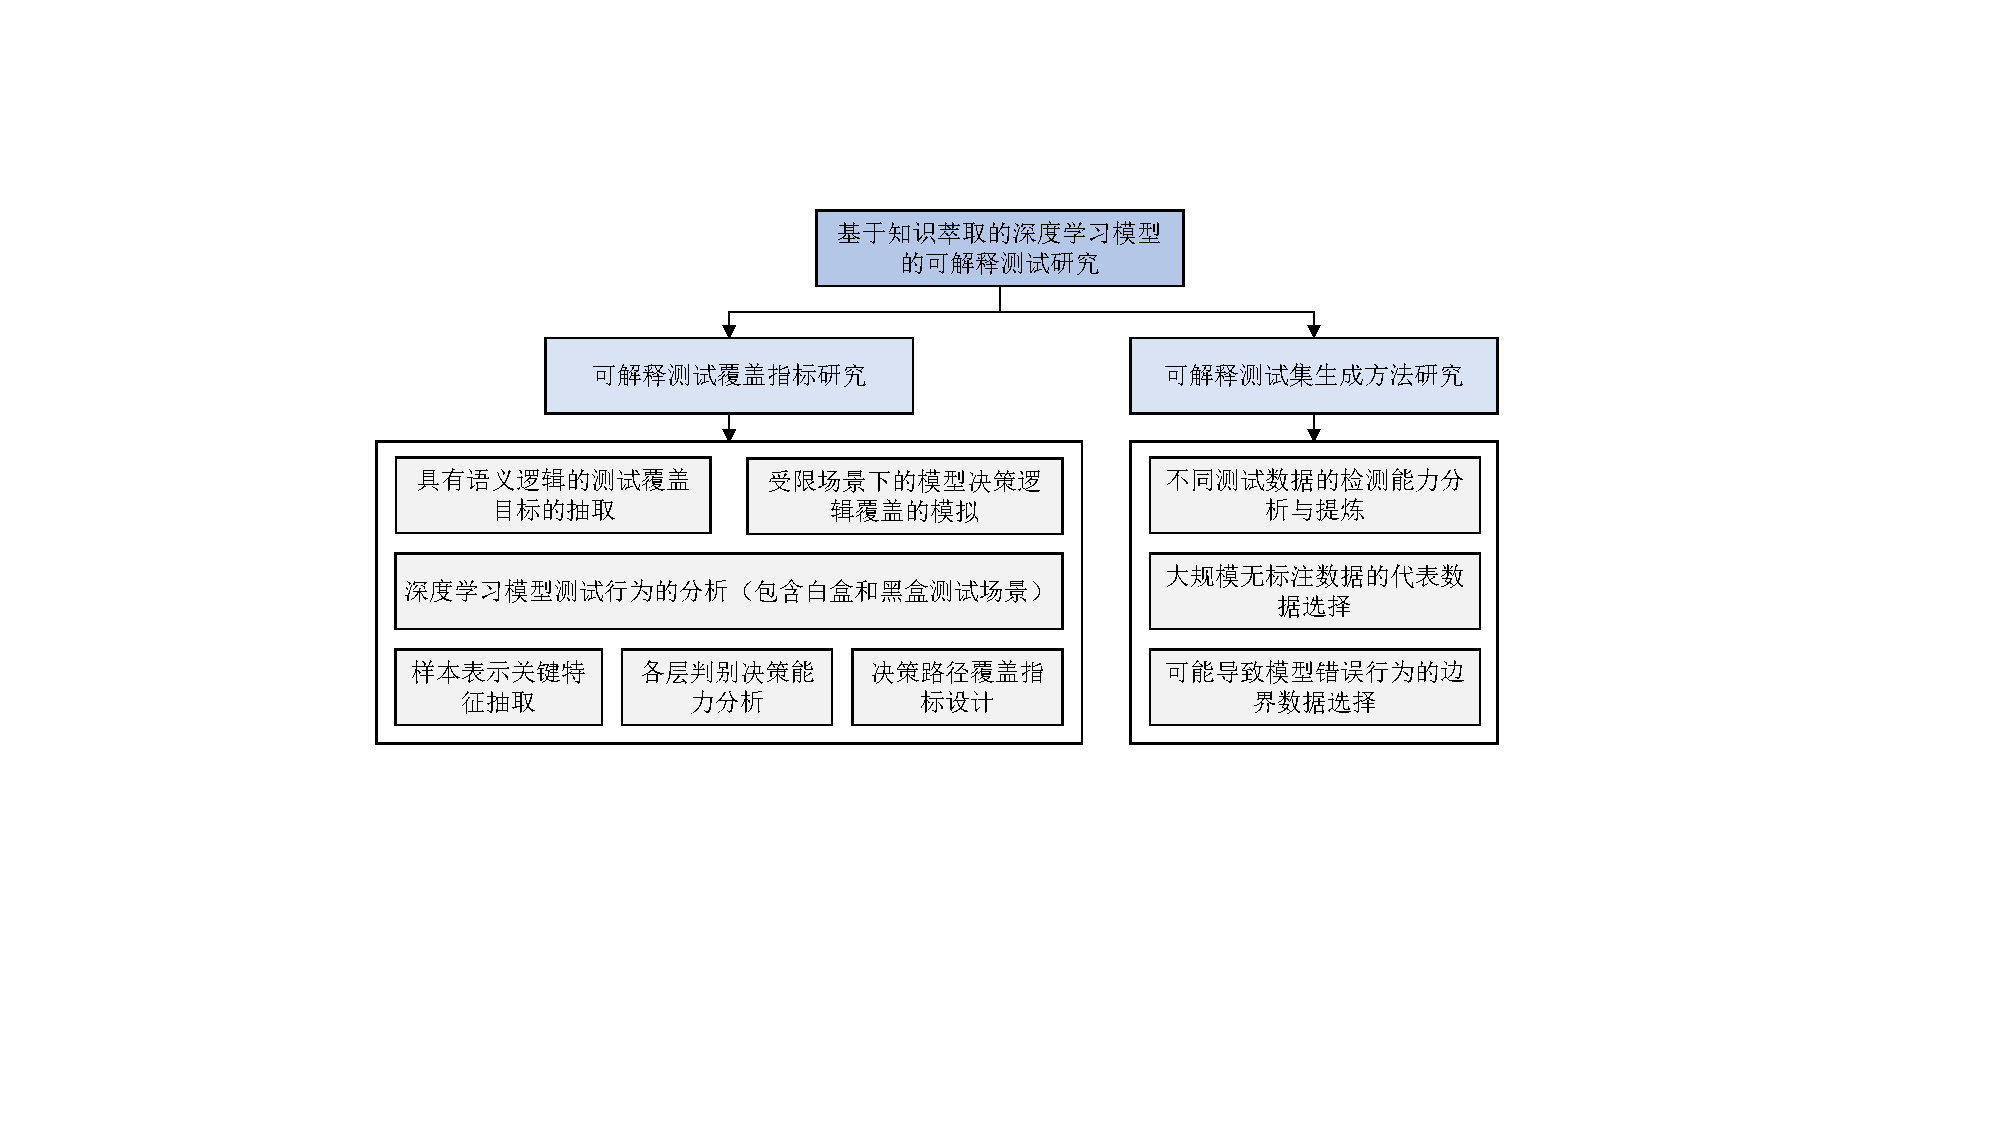
\includegraphics[width=0.85\textwidth]{yjnr.pdf}
        \end{center}
        \caption{挑战、科学问题和研究内容关系图}
        \label{fig:ch2:yjnr}
    \end{small}
\end{figure}

\subsubsection{可解释测试覆盖指标研究}
根据国内外研究现状,现有的深度学习模型测试方法的可解释性十分有限,相关研究工作还非常缺乏。\textbf{针对深度学习模型测试方
    法的可解释性研究工作,测试覆盖指标的缺乏可解释性是显著的挑战之一,也是难点之一}。测试覆盖指标缺乏可解释性导致:a)以
提高测试覆盖率为目标的深度学习测试方法缺乏明显的测试逻辑;b)测试数据的覆盖特征向量无法体现模型的决策路径和决策依据,
很难通过测试执行情况来检查模型是否在以符合人类认知的形式正常工作;c)测试结果缺乏可解释性,测试人员无法知道测试执行失
效的原因,因此无法根据测试结果来辅助诊断模型缺陷。因此,亟待开展针对深度学习模型的可解释测试覆盖指标研究,并在此基础
上展开以下技术研究工作:\textbf{a)研究针对深度学习模型隐藏层的测试语义抽取技术;b)研究在受限场景下的决策逻辑模拟
    技术;c)研究可解释的测试覆盖指标构建方法。}针对测试覆盖指标的可解释性研究作为深度学习模型测试的可解释性研
究的基础,对可解释测试方法的设计与实现中多个关键技术有十分重要的支撑作用。

\subsubsection{可解释测试集生成技术研究}
由于深度学习模型的输入空间通常存在大量无标注数据,如何从这些数据中选取更有价值的测试数据进行标注和测试,合理平衡测试集的
规模和质量,是测试集生成技术的主要研究内容。根据国内外研究现状,现有的针对深度学习模型的测试集生成方法缺乏容易被测试人员
和用户理解的测试逻辑,测试人员无法解释测试集的充分性和代表性,用户在不了解测试集的情况下很难根据测试覆盖率等指标对模型产
生足够的信任。因此,亟待开展对深度学习模型的可解释测试集生成技术的研究,并在此基础上展开以下技术研究工作:\textbf{a)研究
    测试数据的检测能力分析方法;b)研究大规模无标注数据的代表数据选择技术;c)研究具有可解释性的边界数据选择技术。}通过可解释的
    测试覆盖指标和测试集生成方法,实现一种针对深度学习模型的自动化、可解释的测试方法。


\subsection{拟解决的关键科学问题}

如\Cref{fig:ch2:rc}所示,基于上述研究目标和主要研究内容,本项目需要针对以下关键
科学问题进行逐一探索和解决。

\begin{figure}[htp]
    \begin{small}
        \begin{center}
            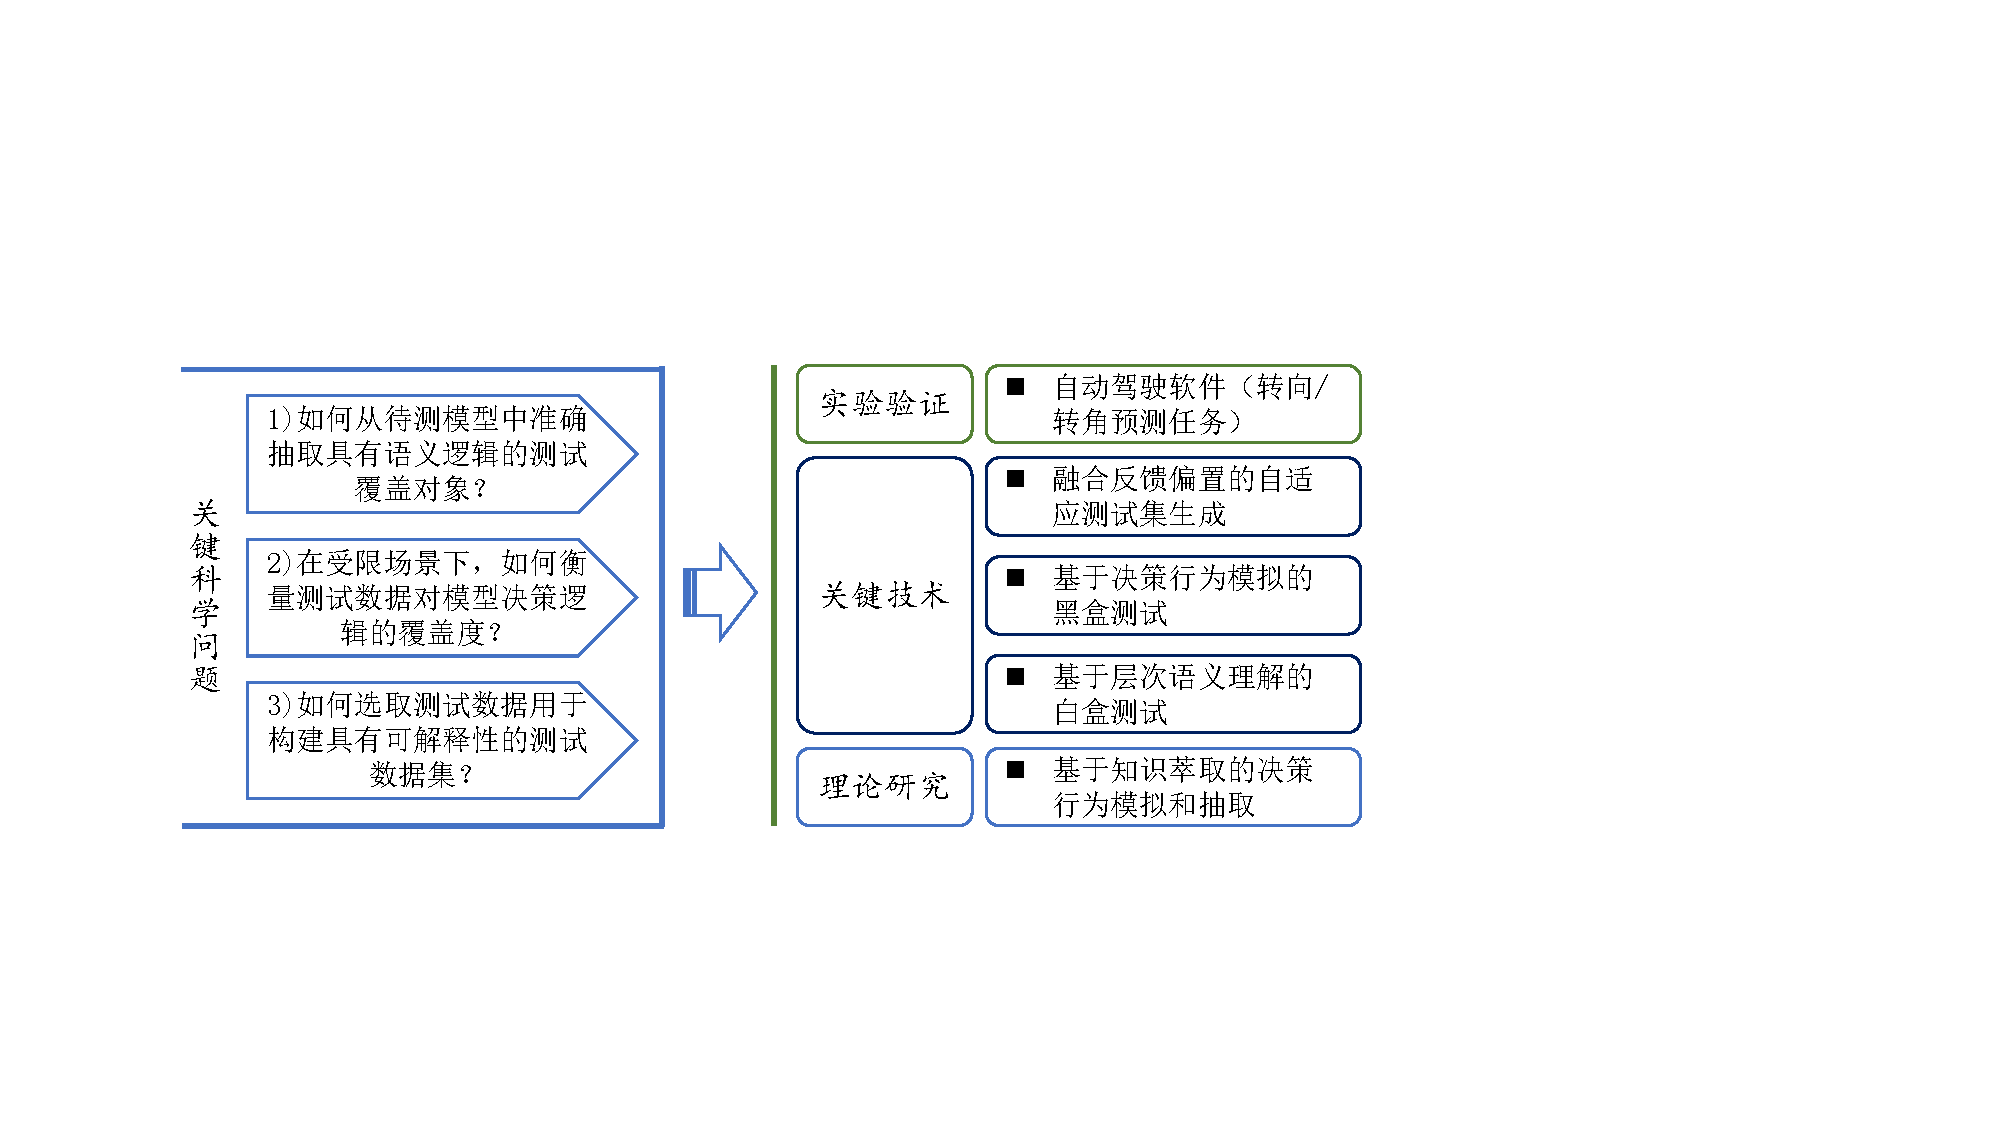
\includegraphics[width=0.95\textwidth]{ch2_RC.pdf}
        \end{center}
        \caption{挑战、科学问题和研究内容关系图}
        \label{fig:ch2:rc}
    \end{small}
\end{figure}

\subsubsection{如何从待测模型中准确抽取具有语义逻辑的测试覆盖对象?}

语义逻辑抽取是构建针对深度学习模型的可解释测试覆盖指标的基础。在可解释测试覆盖指
标的构建中,一方面需考虑测试覆盖对象的语义逻辑,将测试覆盖对象与具有明确语义的模
型行为相联系;另一方面,需克服大规模深度学习模型对可解释性带来的挑战,实现在大规
模深度学习模型的测试应用。现有针对深度学习模型的测试覆盖指标存在覆盖对象缺乏语义
逻辑、伸缩性差的共性问题,难以满足深度学习模型测试的实际应用。因此,如何抽取具有
语义逻辑的测试覆盖对象,自动从深度学习模型的隐藏层中抽取出决策覆盖模式,是定义可
解释的测试覆盖指标亟待解决的关键科学问题。


\subsubsection{在受限场景下,如何衡量测试数据对模型决策逻辑的覆盖度?}
现有测试覆盖指标依赖于测试者掌握所有训练数据和整个深度学习模型,但在受限场景下,
测试者无法访问训练数据和模型的内部结构,因此无法直接抽取模型的决策逻辑和决策依
据。目前针对深度学习模型仅有的黑盒测试研究主要是与模型无关的测试数据多样性度量,
缺乏对模型决策逻辑和决策依据的理解。因此,亟需深入研究仅根据测试数据的输入输出,
衡量测试数据对模型待测功能的覆盖程度,建立基于决策路径模拟的黑盒测试覆盖度指标,
为在受限场景下的深度学习模型可解释测试提供关键技术支撑。


\subsubsection{如何选取测试数据用于构建具有可解释性的测试数据集?}
关键科学问题(1)和(2)解决的是可解释测试覆盖指标的构建,而高质量、可解释的测试
集是准确评估模型性能,也是提高模型可信度的重要保障。一方面,测试数据的标签依赖于
人工标注,成本较高且受限于专家经验,需要合理地平衡测试集的规模与能力;另一方面,
测试数据的选取需要考虑其对真实数据分布的代表性以及在边界数据对模型正确性的影响。
因此,如何自动构建针对深度学习模型的测试集,让测试人员和用户理解测试集的代表性和
充分性,是构建深度学习模型的可解释性测试方法的关键所在。

\iffalse
    \begin{figure}[htp]
        \begin{small}
            \begin{center}
                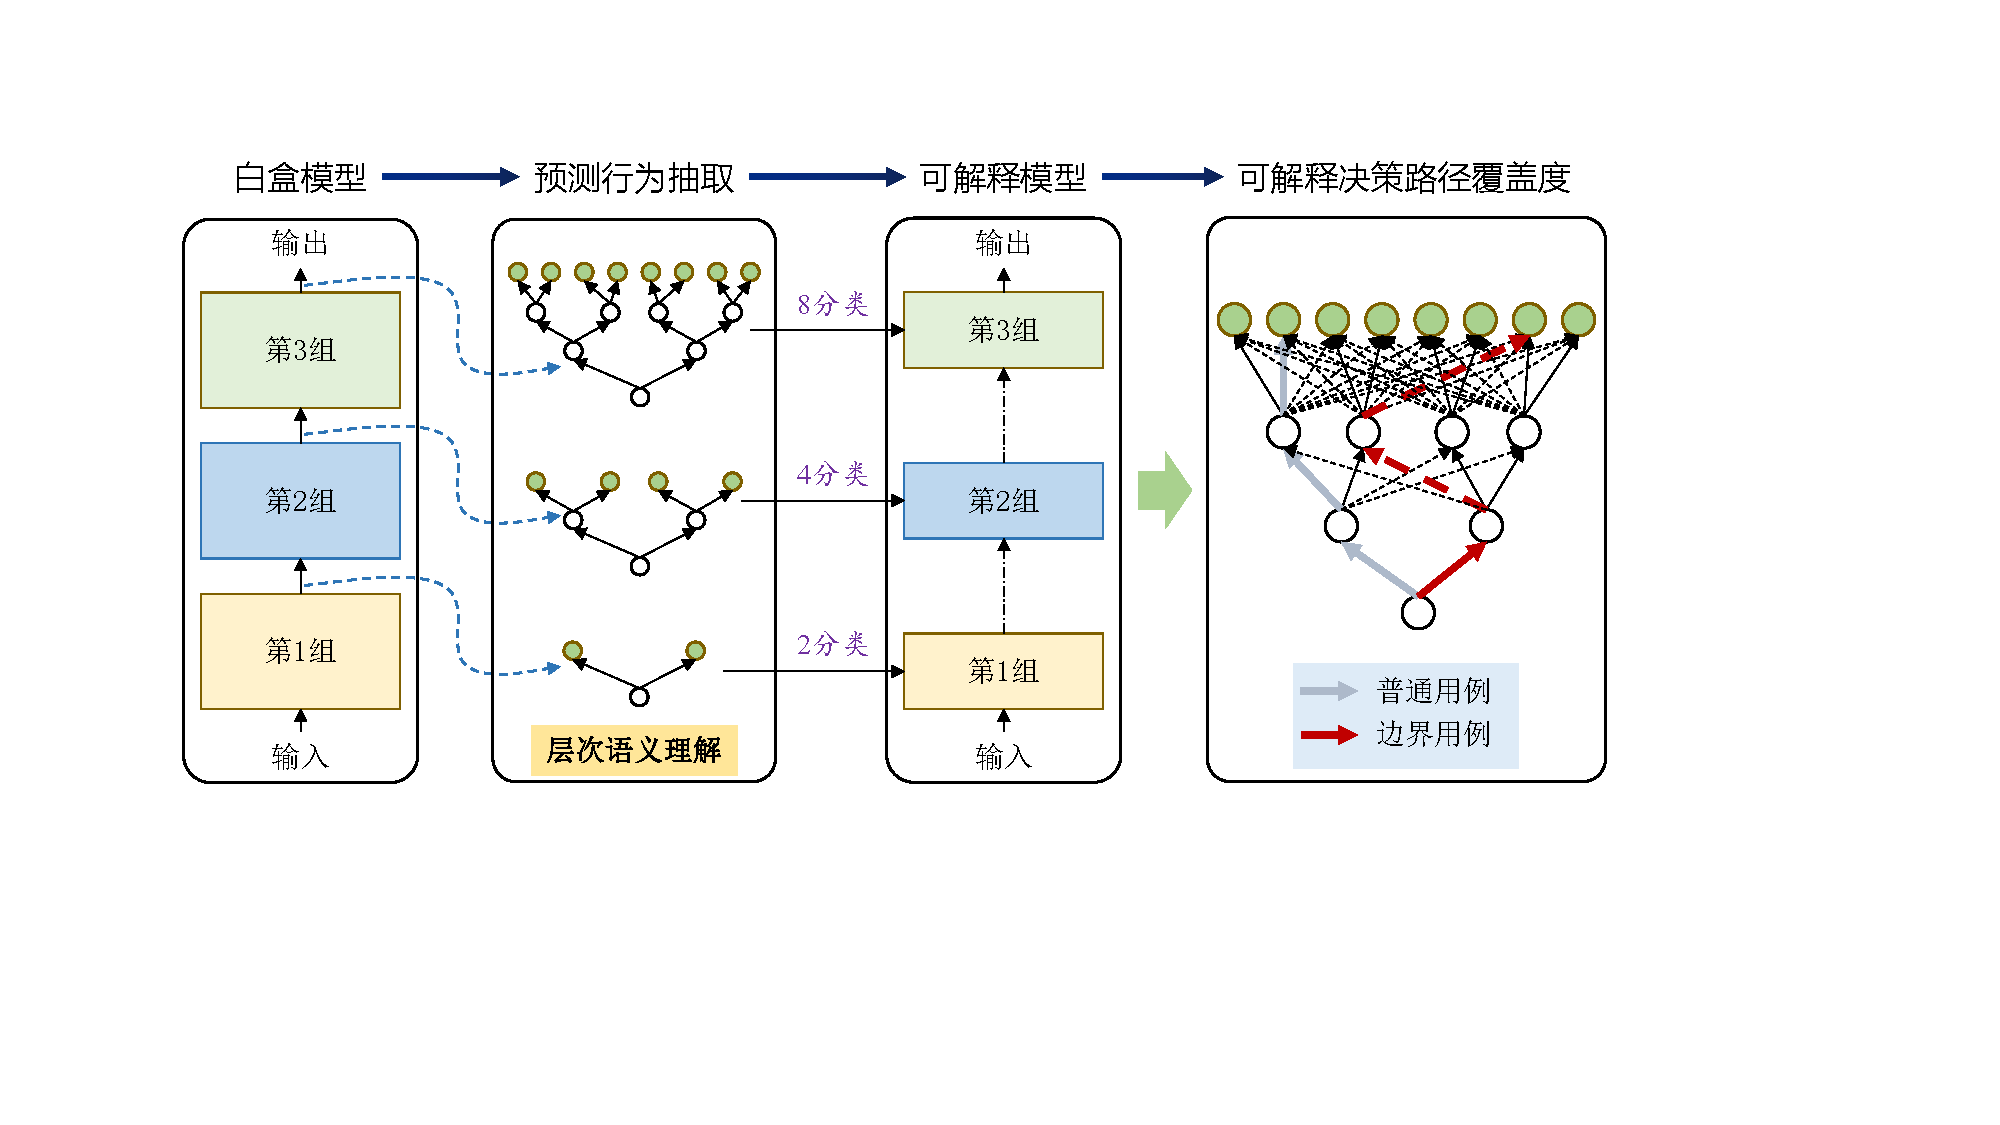
\includegraphics[width=0.9\textwidth]{ch2_WBtest.pdf}
            \end{center}
            \caption{基于层次语义理解的白盒测试研究内容}
            \label{fig:ch2:WBtest}
        \end{small}
    \end{figure}


    \begin{figure}[htp]
        \begin{small}
            \begin{center}
                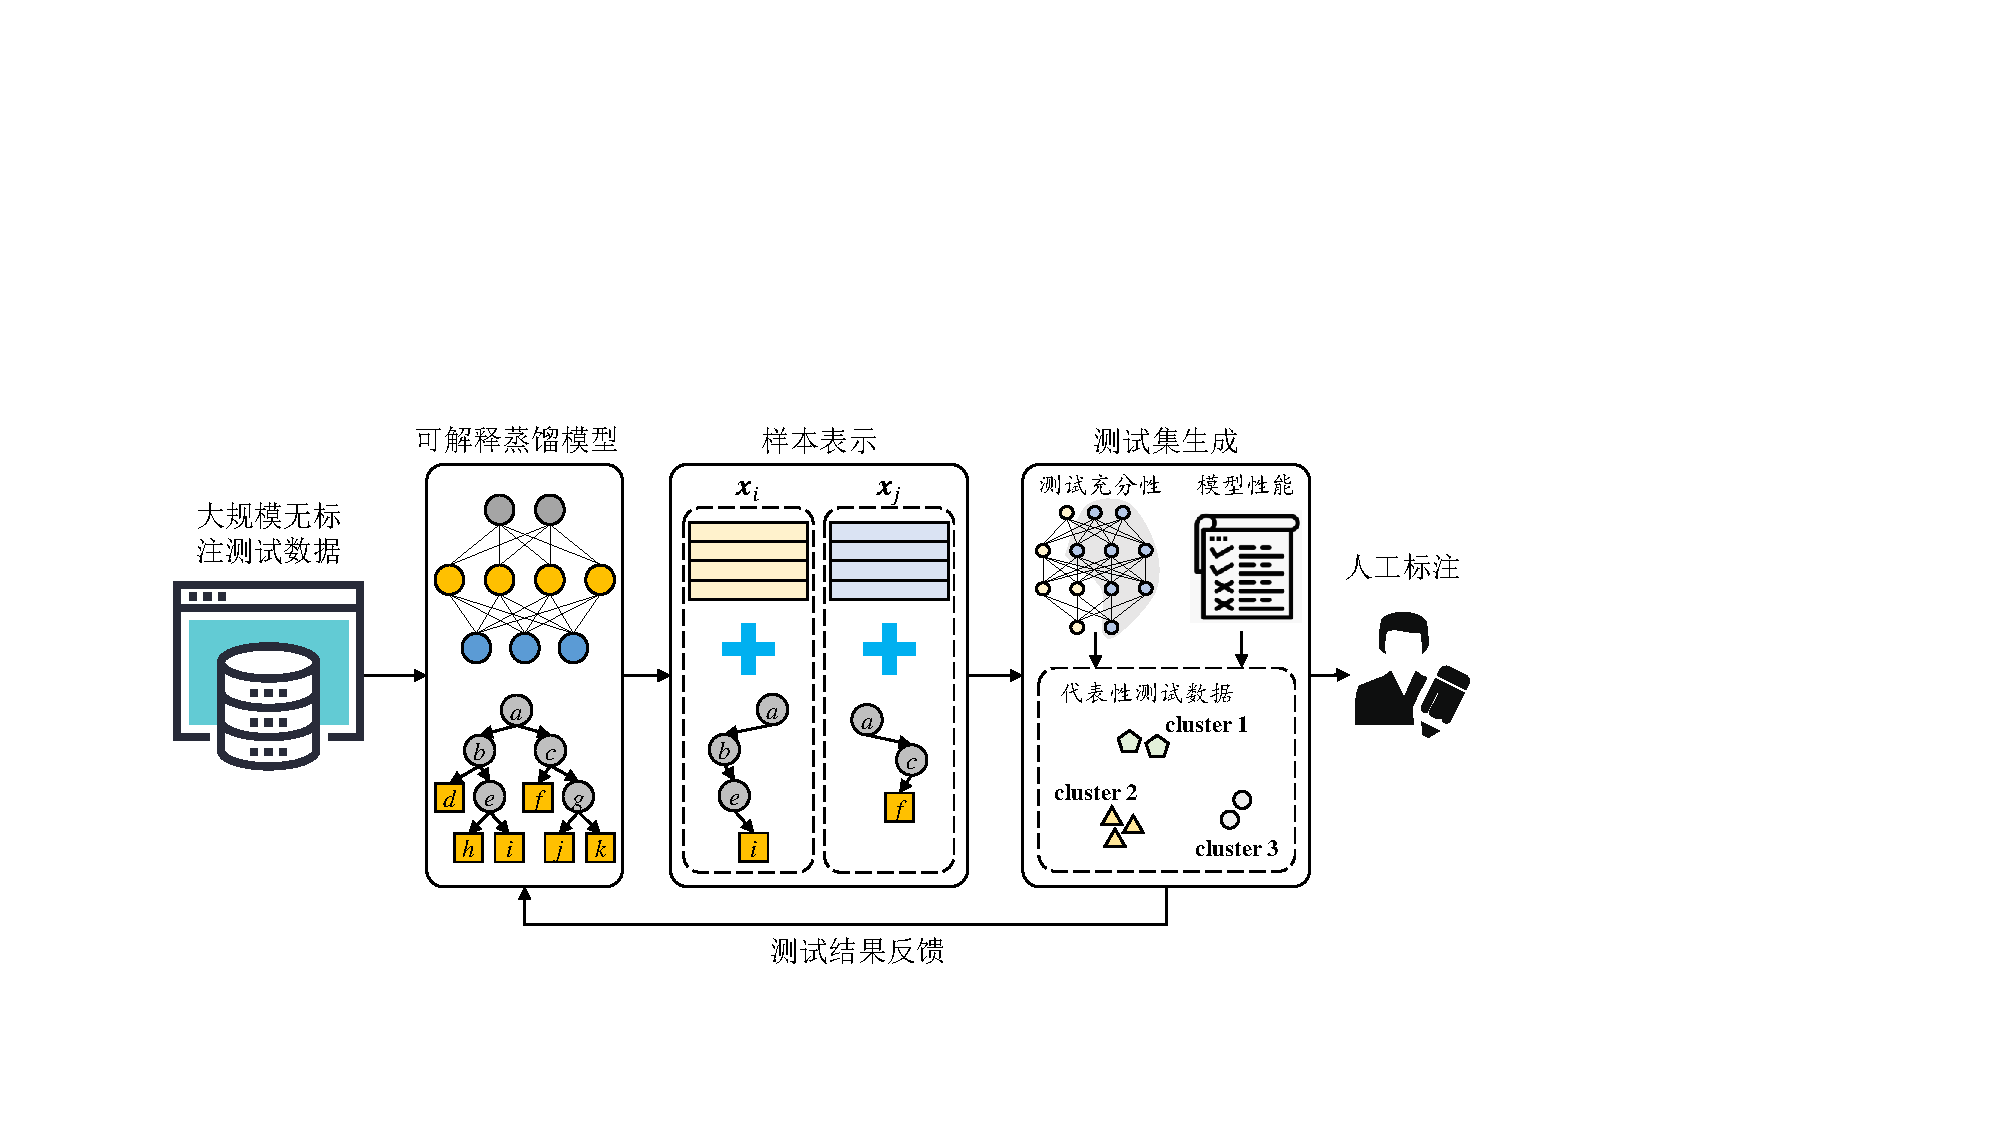
\includegraphics[width=0.95\textwidth]{ch2_TestSelection.pdf}
            \end{center}
            \caption{可解释预测模型研究内容}
            \label{fig:ch2:testselection}
        \end{small}
    \end{figure}

\fi